\chapter{Analysis and Conception}
\label{chapter:design}

\section{Overview}
The vFireLib library provides functions that allow for a dynamic forest fire simulation to occur. The library is responsible for managing the data provided by input files by a user, calculating spread data, running the sequential or parallel simulation, and writing out the final data to a file for further reading. The diagrams in this section of the paper were generated using the Creately web interface for generating UML diagrams \cite{creately}. 

\section{Service Requirements}

\subsection{Functional Requirements}
The functional requirements were created from the behavioral requirements of the library's functionality as used by an outside source. The list of functional requirements may be viewed in Table \ref{tbl:functional_reqs}.

\begin{table}
\caption{vFireLib Wildfire Simulation Library Functional Requirements.}
\label{tbl:functional_reqs}
  \rowcolors{2}{gray!25}{white}
  \begin{tabular}{cl}
    \rowcolor{gray!50}
    Number & Description \\
    FR01 &  \begin{tabular}[c]{@{}l@{}}The library shall read in fuel model, moisture model, and\\ terrain data.\end{tabular}\\
    FR02 & The library shall define the granularity of simulation size. \\
    FR03 &  \begin{tabular}[c]{@{}l@{}}The library shall create and initialize all data members necessary\\ to a complex simulation on the CPU and GPU.\end{tabular}\\
    FR04 & The simulation shall calculate the maximum rate of spread for every cell. \\
	FR05 & \begin{tabular}[c]{@{}l@{}}The library shall run a GPU simulation using the BD, MT,\\ or IMT spread methodologies. \end{tabular}\\
    FR06 & The library shall calculate fire acceleration for the simulation. \\
    FR07 & The library shall allow the Crowning flag to be toggled. \\
    FR08 & The library shall allow the Spotting flag to be toggled. \\
    FR09 & \begin{tabular}[c]{@{}l@{}}The library notify the user when their input files are not compatible\\ with the simulation system. \end{tabular}\\
    FR010 & The data must be initialized before the simulation is run. 
  \end{tabular}
 % \end{table}
%\begin{table}
\\ \\
\caption{vFireLib Wildfire Simulation Library Non-functional Requirements.}
\label{tbl:nonfunctional_reqs}
  \rowcolors{2}{gray!25}{white}
  \begin{tabular}{cl}
    \rowcolor{gray!50}
    Number & Description \\
    NR01 & The library shall be written in C++ and CUDA. \\
    NR02 & The library must use CUDA version 6.0 or higher. \\
    NR03 & \begin{tabular}[c]{@{}l@{}}The library's sequential implementation must be a direct reflection of its\\ parallel implementation. \end{tabular}\\
    NR04 & \begin{tabular}[c]{@{}l@{}}To run the parallel version of the code, an NVIDIA GPU with CUDA Compute\\ Capability 2.0 or higher is needed. \end{tabular}\\
    NR05 & This library must be used on the Linux platform. \\
    NR06 & The library must use GDAL version 1.10.1. \\
    NR07 & The library must be compiled with CMake Version 2.8 or higher. \\
  \end{tabular}
  \end{table}

\subsection{Non-functional Requirements}
The non-functional requirements were created based on the internal interactions of the library functions. Data needed to be manipulated and passed among classes and between the host and device for computation purposes. The non-functional requirements are listed in Table \ref{tbl:nonfunctional_reqs}.
  
\section{Use Case Modeling}
\subsection{Overview}
For a better understanding of how the user interacts with the library, this section describes use cases for running a simulation. Both the parallel and sequential functionalities will be shown here. The use case model may be found in Figure \ref{fig:usecase_diagram}. In order to better illustrate the library's functionality, a sequence diagram may be seen in Figure \ref{fig:sequence_diagram}. 

\begin{figure}
    \centering
    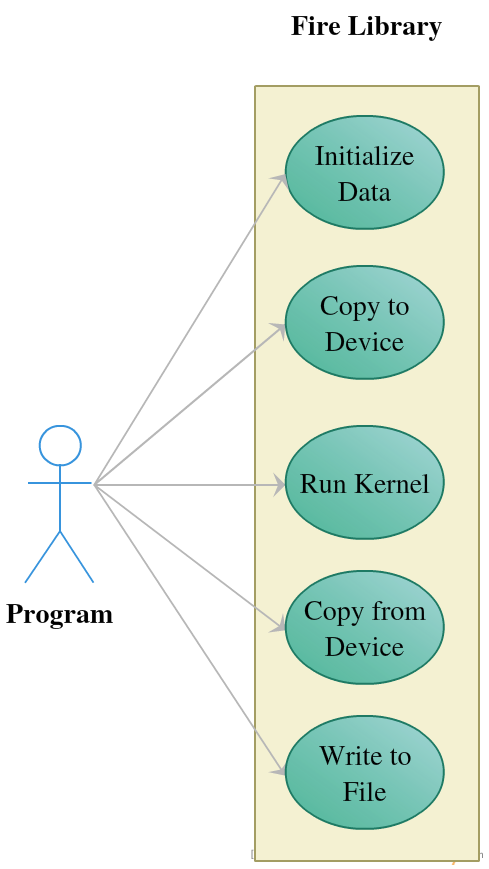
\includegraphics[height=4.5in,width=\textwidth,keepaspectratio]{figures/design/use_case_diagram.png}
    \caption{A use case diagram for the Wildfire simulation library.}
    \label{fig:usecase_diagram}
\end{figure}

\begin{figure}
    \centering
    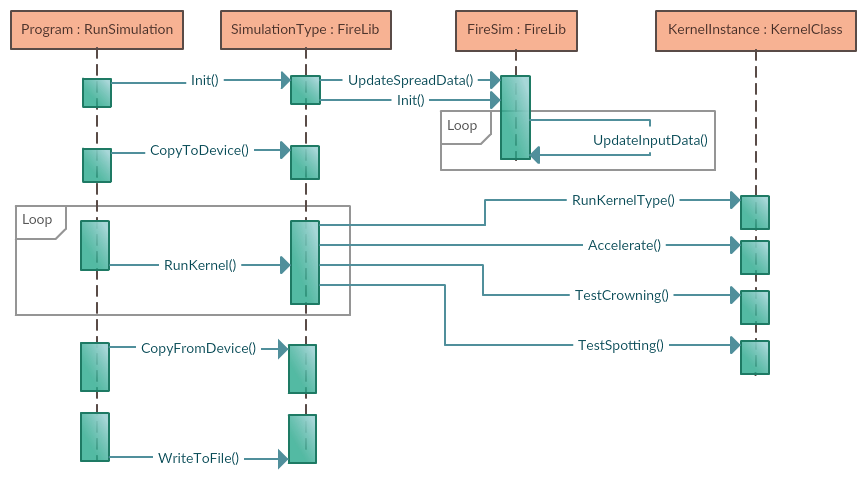
\includegraphics[height=\textheight,width=\textwidth,keepaspectratio]{figures/design/sequence_diagram.png}
    \caption{A sequence diagram for the Wildfire simulation library.}
    \label{fig:sequence_diagram}
\end{figure}

\subsection{Detailed Use Cases}
\subsubsection{Initialize Simulation Data}
The terrain data encompasses more than the terrain data. The fuel model data must be read from the files, the terrain data, the moisture data, the canopy height data, the crown base height data, and the crown bulk density data. If there is an error with any of these files, the library reports an error. This is the point where the simulation is scaled to the appropriate granularity. 

\subsubsection{Initialize CPU Data}
The data must be initialized from the input data into a format which is useable by the simulation. This includes calculating the maximum spread rate before the simulation begins. This function must be called whenever there is a change to the data values in the initialize function. 

\subsubsection{Copy To Device}
The data needed for the simulation must be copied from the host to the device (GPU). This must occur every time the data is changed on the CPU side of the library. 

\subsubsection{Propagate}
This occurs when a propagate function is called. This could be from three sources: BD, MT, or IMT. 

\subsubsection{Accelerate}
Once the fire has spread after a time tick, the rate of spread from the fire is accelerated.

\subsubsection{Crowning}
Once the fire has been accelerated, a test is done to see if the fire is crowning. The moment a fire crowns, the torching flag is set for one time tick. The crowning test also checks to see if the fire is passive. If it has progressed to an active fire, the maximum rate of spread is updated to reflect the change. 

\subsubsection{Spotting}
In the event that torching has occurred during the crowning phase, spotting is calculated. A fire brand is launched into the air and it is tested to calculate if any new fires start ahead of the flame wall.

\subsubsection{Copy From Device}
On completion of the desired simulation, the data from the simulation must be copied back from the device back to the host for further processing. 

\subsubsection{Write To File}
This functionality allows the user to write the computed output of their time of arrival map to a .csv output file. 

\section{Architecture}
This library is designed to act as a facilitation tool that will allow a user to program their own custom-defined simulations. The program aims to make visualization easily portable to users. In order to convey an understanding of the overall architecture of the library, a class diagram is provided to describe the system in Figures \ref{fig:class_diagram} and \ref{fig:fire_sim_class_diagram}:

\begin{figure}
    \centering
    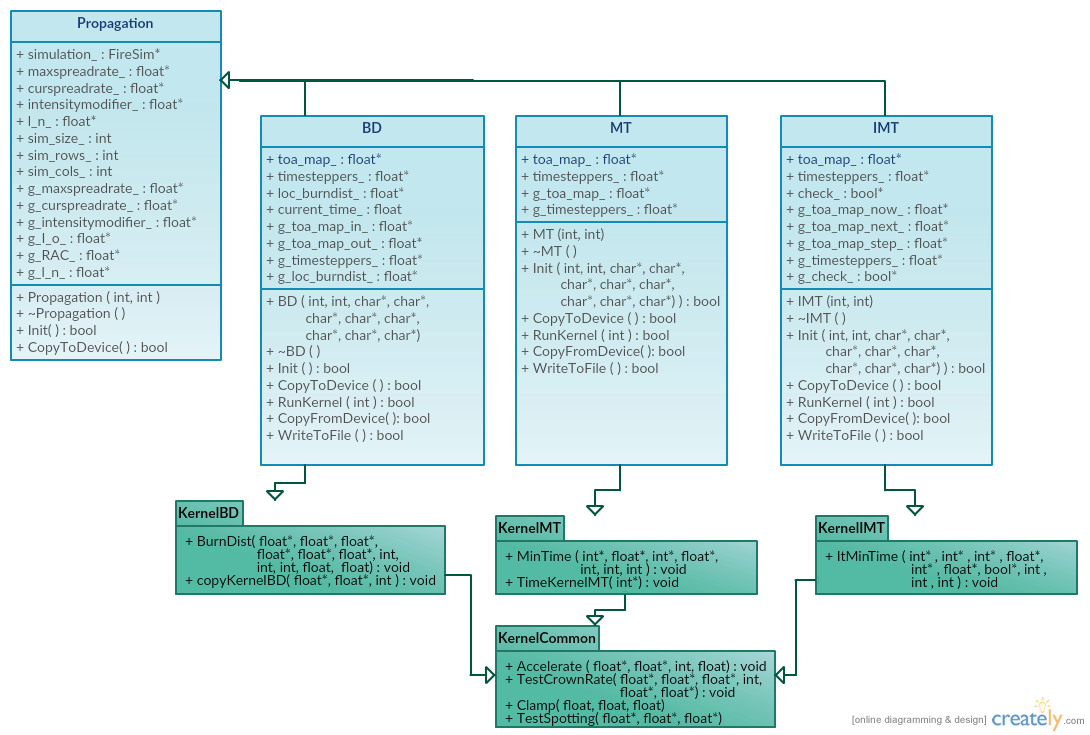
\includegraphics[width=\textwidth,keepaspectratio]{figures/design/class_diagram.png}
    \caption{A class diagram for the Propagation classes in the simulation library.}
    \label{fig:class_diagram}
\end{figure}

\begin{figure}
    \centering
    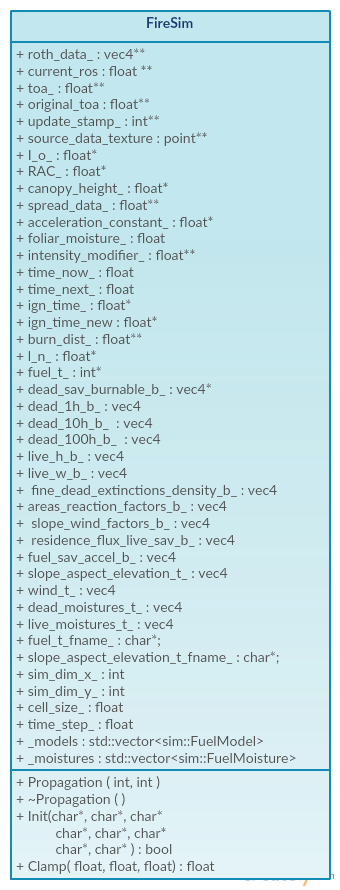
\includegraphics[height=\textheight,keepaspectratio]{figures/design/fire_sim_diagram.png}
    \caption{A class diagram for the Propagation classes in the simulation library.}
    \label{fig:fire_sim_class_diagram}
\end{figure}
